\documentclass[11pt]{scrartcl}
\usepackage[T1]{fontenc}
\usepackage[a4paper, left=3cm, right=2cm, top=2cm, bottom=2cm]{geometry}
\usepackage[activate]{pdfcprot}
\usepackage[ngerman]{babel}
\usepackage[parfill]{parskip}
\usepackage[utf8]{inputenc}
\usepackage[math]{kurier}
\usepackage{amsmath}
\usepackage{amssymb}
\usepackage{xcolor}
\usepackage{epstopdf}
\usepackage{txfonts}
\usepackage{fancyhdr}
\usepackage{graphicx}
\usepackage{prettyref}
\usepackage{hyperref}
\usepackage{eurosym}
\usepackage{setspace}
\usepackage{units}
\usepackage{eso-pic,graphicx}
\usepackage{icomma}
\usepackage{pdfpages}

\definecolor{darkblue}{rgb}{0,0,.5}
\hypersetup{pdftex=true, colorlinks=true, breaklinks=false, linkcolor=black, menucolor=black, urlcolor=darkblue}



\setlength{\columnsep}{2cm}


\newcommand{\arcsinh}{\mathrm{arcsinh}}
\newcommand{\asinh}{\mathrm{arcsinh}}
\newcommand{\ergebnis}{\textcolor{red}{\mathrm{Ergebnis}}}
\newcommand{\fehlt}{\textcolor{red}{Hier fehlen noch Inhalte.}}
\newcommand{\betanotice}{\textcolor{red}{Diese Aufgaben sind noch nicht in der Übung kontrolliert worden. Es sind lediglich meine Überlegungen und Lösungsansätze zu den Aufgaben. Es können Fehler enthalten sein!!! Das Dokument wird fortwährend aktualisiert und erst wenn das \textcolor{black}{beta} aus dem Dateinamen verschwindet ist es endgültig.}}
\newcommand{\half}{\frac{1}{2}}
\renewcommand{\d}{\, \mathrm d}
\newcommand{\punkte}{\textcolor{white}{xxxxx}}
\newcommand{\p}{\, \partial}
\newcommand{\dd}[1]{\item[#1] \hfill \\}

\renewcommand{\familydefault}{\sfdefault}
\renewcommand\thesection{}
\renewcommand\thesubsection{}
\renewcommand\thesubsubsection{}


\newcommand{\themodul}{Konstruktionstechnik Formelsammlung V1.0}
\newcommand{\thetutor}{}
\newcommand{\theuebung}{}

\pagestyle{fancy}
\fancyhead[L]{\footnotesize{C. Hansen}}
\chead{\thepage}
\rhead{}
\lfoot{}
\cfoot{}
\rfoot{}

\title{\themodul{}}


\author{Christoph Hansen \\ {\small \href{mailto:chris@university-material.de}{chris@university-material.de}} }

\date{}


\begin{document}

\maketitle

Dieser Text ist unter dieser \href{http://creativecommons.org/licenses/by-nc-sa/4.0/}{Creative Commons} Lizenz veröffentlicht.

\textcolor{red}{Ich erhebe keinen Anspruch auf Vollständigkeit oder Richtigkeit. Falls ihr Fehler findet oder etwas fehlt, dann meldet euch bitte über den Emailkontakt.}


Die Bilder sind aus dem KT Skript von Herrn Stellberg entnommen. Das Urheberrecht liegt bei ihm!

\tableofcontents


\newpage

\section{Widerstandsmomente}

\begin{figure}[h]
	\centering
	%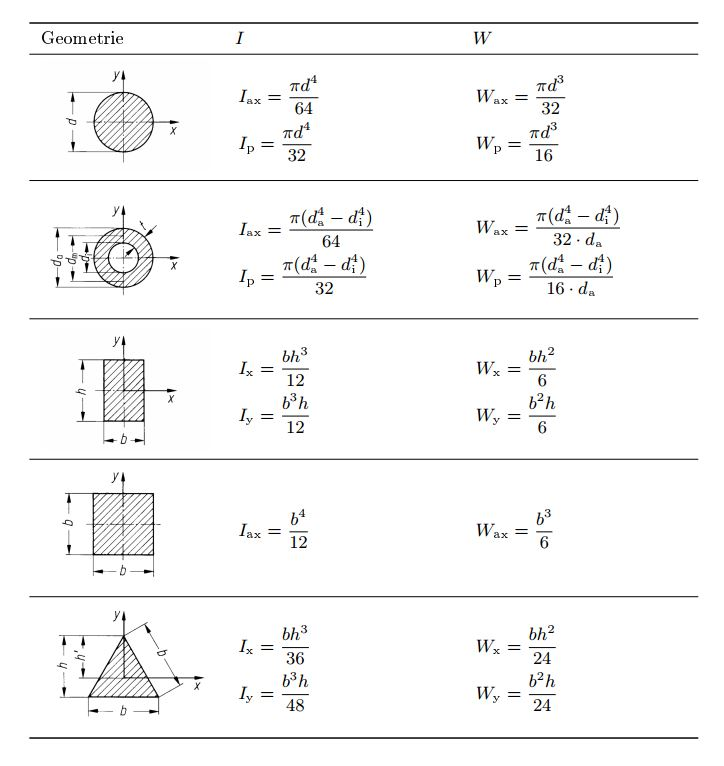
\includegraphics[scale=0.9]{Widerstandsmomente.jpg}
	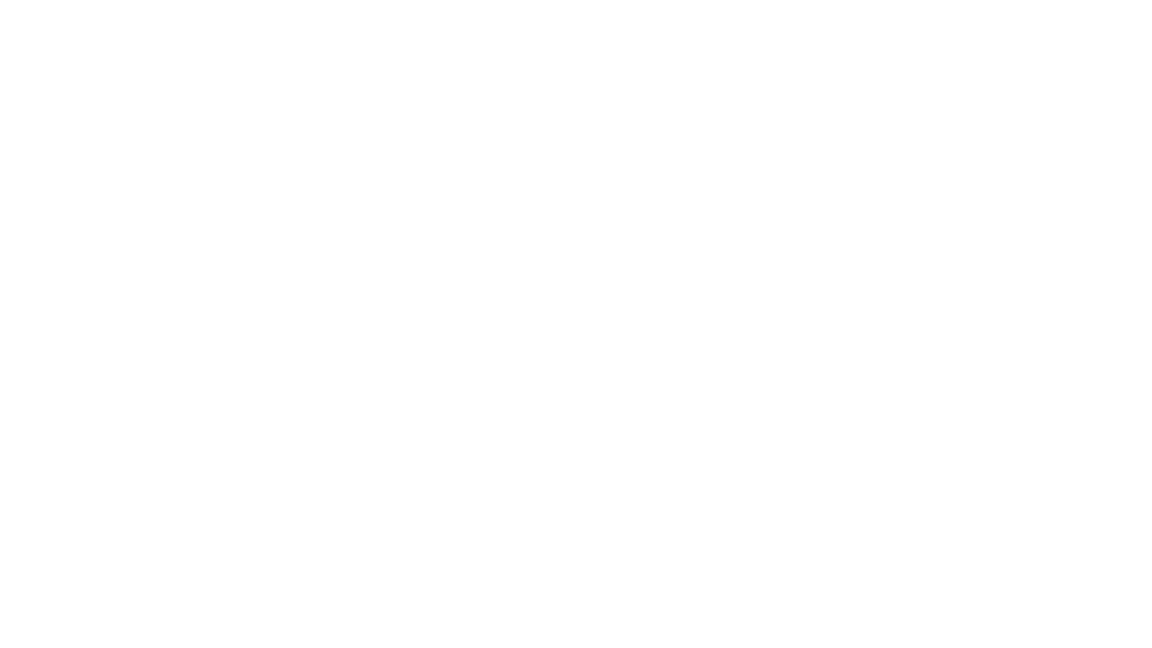
\includegraphics[scale=0.9]{leer.png}
	\caption{Widerstandsmomente aus Römerturm}
\end{figure}


\newpage


\section{Beanspruchung}

\begin{align*}
\intertext{Spannung im Balken:}
\sigma &= \frac{F}{A} = Re_p
\intertext{Trägheitsradius:}
i &= \sqrt{\frac{I}{A}} \qquad \text{I = Axials Flächenträgheitsmoment, A = Querschnittfläche}
\intertext{Schlankheitsgrad:}
\lambda &= \frac{l_k}{i} \qquad \text{$l_k$ = Knicklänge}
\intertext{Knicklänge:}
l_k &= k \cdot L_0
\end{align*}

\begin{figure}[h]
	\centering
	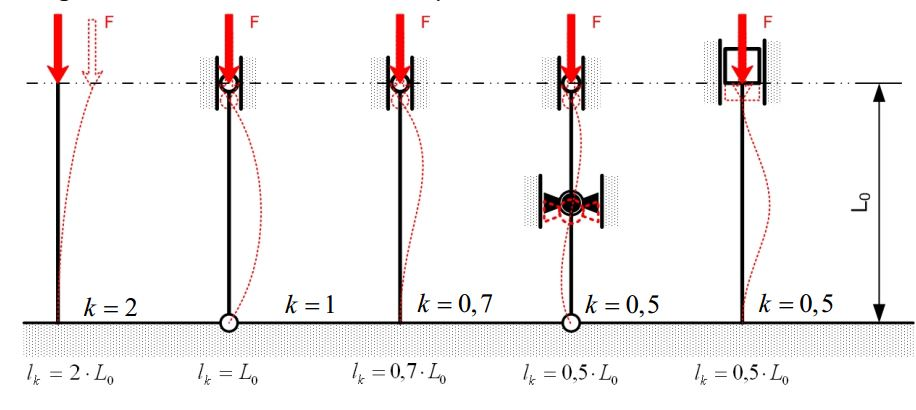
\includegraphics[scale=0.7]{Einspannfaelle.jpg}
\end{figure}

\begin{align*}
F_{KE} &= \frac{E \cdot I \cdot \pi^2}{l_k^2} \\ 
\intertext{E = Elas. mod., I = min. axiales Flächenträgheitsmoment}
\intertext{Drucknennspannung bei Knickkraft:}
\sigma_k &= \frac{\pi^2 \cdot E}{\lambda^2}
\intertext{Grenzschlankheitsgrad:}
\lambda_p &= \sqrt{\frac{\pi^2 \cdot E}{Re_p}}
\end{align*}

\subsection*{Schubmittelpunk}


Es gibt folgende Standard Schubmittelpunk Formeln:

\begin{figure}[h]
	\centering
	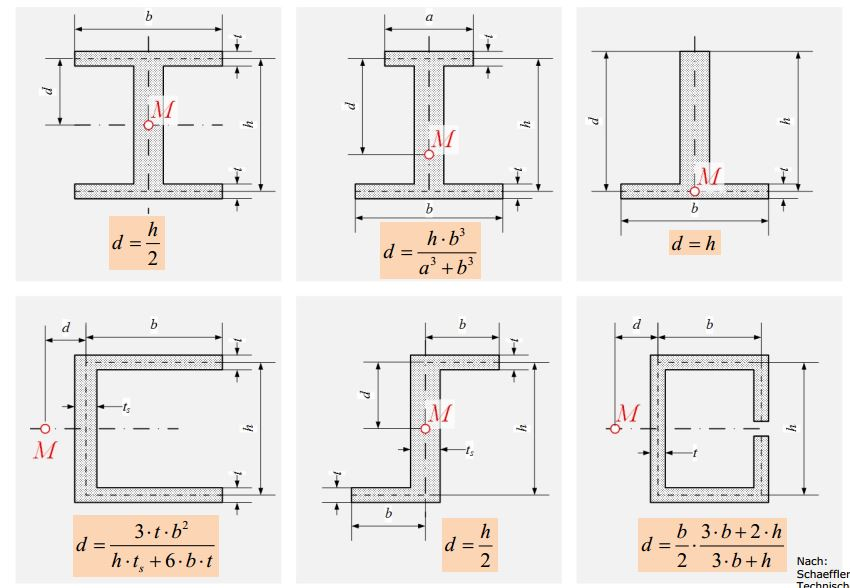
\includegraphics[scale=0.7]{Schubmittelpunk_1.jpg}
\end{figure}

\begin{figure}[h]
	\centering
	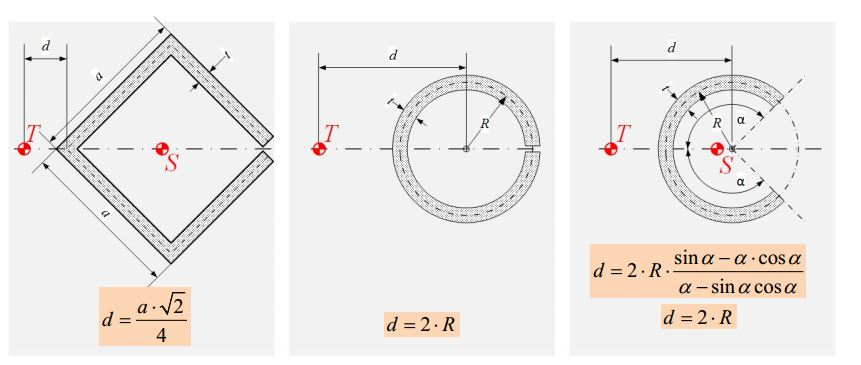
\includegraphics[scale=0.7]{Schubmittelpunk_2.jpg}
\end{figure}

\newpage

Bei jedem anderen Körper rechnet man wie folgt:

\begin{figure}[h]
	\centering
	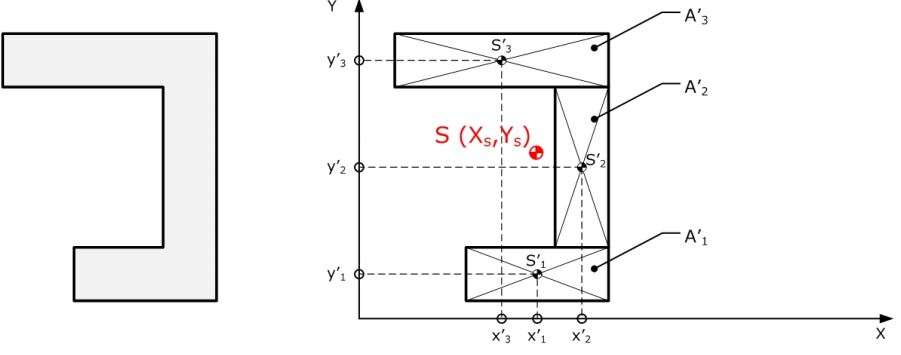
\includegraphics[scale=0.7]{Schubmittelpunk_Rechnung.jpg}
\end{figure}

\begin{align*}
X_S &= \frac{\sum_{1}^{n} x_n' \cdot A_n'}{\sum_{1}^{n} A_n'} \qquad
Y_S = \frac{\sum_{1}^{n} y_n' \cdot A_n'}{\sum_{1}^{n} A_n'} 
\end{align*}

\subsection*{Querkraft}


\begin{figure}[h]
	\centering
	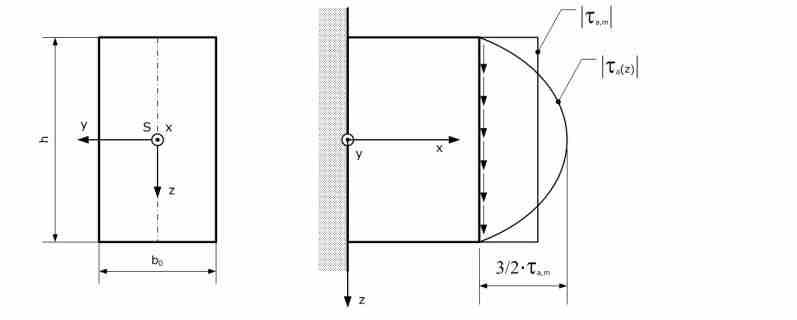
\includegraphics[scale=0.7]{Querkraftschub.jpg}
\end{figure}

\begin{align*}
\tau_{a,m} &= \frac{F}{b_0 \cdot h} \qquad \qquad \tau_a(z) = \frac{3}{2} \cdot \left[ 1 - 4 \cdot \left( \frac{z}{h} \right)^2 \right] \cdot \frac{F}{b_0 \cdot h}
\end{align*}


\subsection*{Torsion}


\begin{align*}
I_t &= \frac{4 \cdot A_m^2}{\int \frac{\d s}{h(s)}}
\intertext{Für Profile mit abschnittweise konstantem $h(s)$ gilt:}
I_t &= \frac{4 \cdot A_m^2}{\sum_{i}^{} \frac{l_i}{h_i}}
\end{align*}



\subsubsection*{Dünnwandige, geschlossene, einzellige Hohlprofile}


\begin{figure}[h]
	\centering
	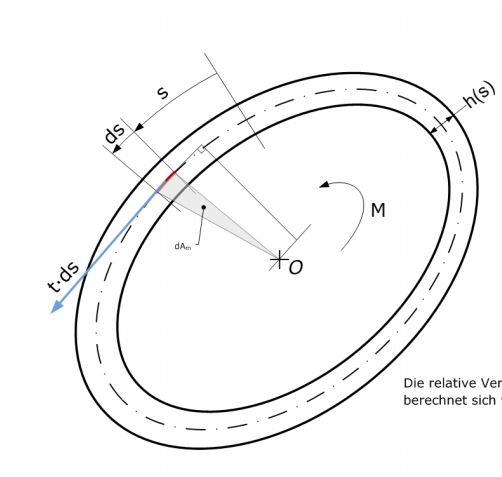
\includegraphics[scale=0.6]{Torsion_1.jpg}
\end{figure}

\begin{align*}
\intertext{Der Schubfluss ist über den Umfang konstant:}
t &= \frac{M}{2 \cdot A_m} = const
\intertext{Torsionsspannung:}
\tau_t(s) &= \frac{t}{h(s)} = \frac{M}{2 \cdot A_m \cdot h(s)} 
\intertext{maximale Torsionsspannung:}
\tau_t(s) &= \frac{t}{h(s)} = \frac{M}{2 \cdot A_m \cdot h_{min}} \qquad \text{mit} \qquad W_t = 2 \cdot A_m \cdot h_{min}
\intertext{Verdrillung:}
\phi &= \frac{M \cdot l}{G \cdot I_t}
\end{align*}


\newpage

\subsubsection*{Dünnwandige, geschlossene Profile}


\begin{figure}[h]
	\centering
	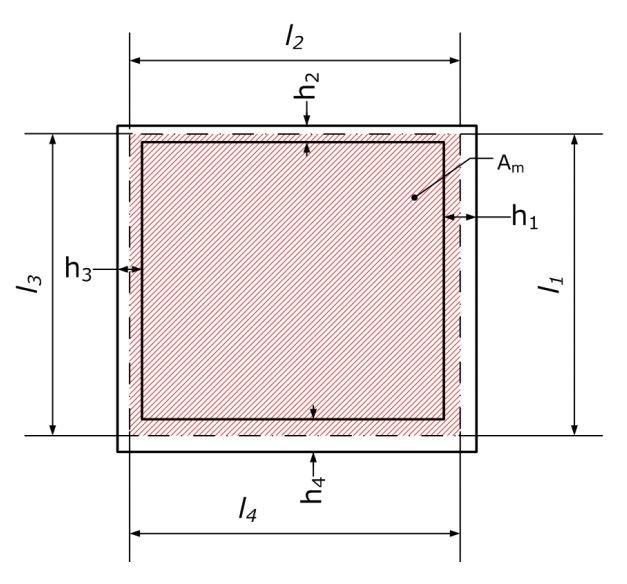
\includegraphics[scale=0.6]{Torsion_2.jpg}
\end{figure}


\begin{align*}
I_t &= \frac{4 \cdot A_m^2}{\frac{l_1}{h_1} + \frac{l_2}{h_2} + \frac{l_3}{h_3} + \frac{l_4}{h_4}}
\end{align*}


\subsubsection*{Dünnwandige, geschlossene Profile}


\begin{figure}[h]
	\centering
	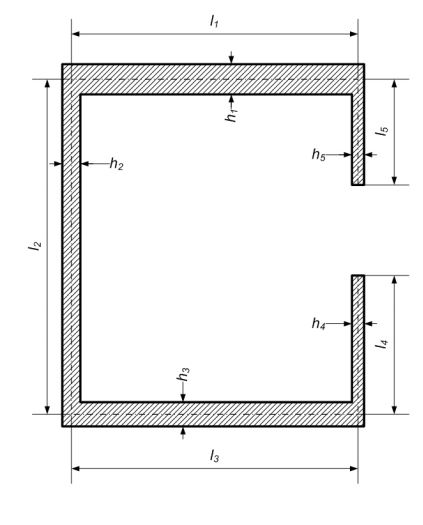
\includegraphics[scale=0.6]{Torsion_3.jpg}
\end{figure}


\begin{align*}
\intertext{maximale Torsionsspannung:}
\tau_{t,max} &= \frac{M}{I_t} \cdot h_{max} \qquad \text{mit} \qquad W_t = \frac{I_t}{h_{max}}
\intertext{Verdrillung:}
\phi &= \frac{M \cdot l}{G \cdot I_t} \\
\hfil \\
I_t &= \frac{1}{3} \cdot \sum_{i}^{} l_i \cdot h_i^3
\end{align*}


\subsubsection*{Geschlitzte Rohre}


\begin{figure}[h]
	\centering
	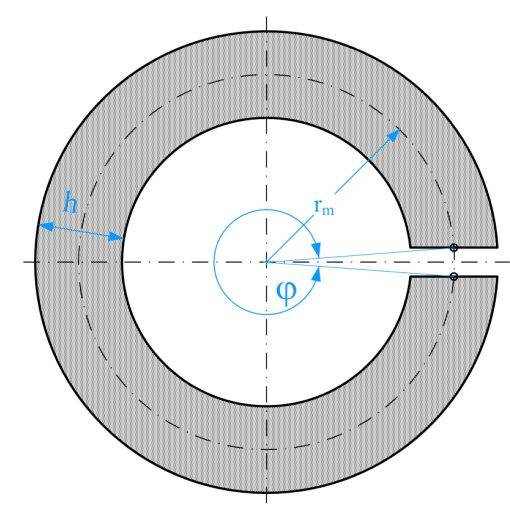
\includegraphics[scale=0.6]{Torsion_4.jpg}
\end{figure}


\begin{align*}
l &= \phi \cdot r \qquad
I_t = \frac{1}{3} \cdot l \cdot h^3 \qquad
W_t = \frac{1}{3} \cdot l \cdot h^2
\end{align*}

\newpage

\subsubsection*{Offene, dünnwandige Profile. Korrekturfaktor.}


\begin{figure}[h]
	\centering
	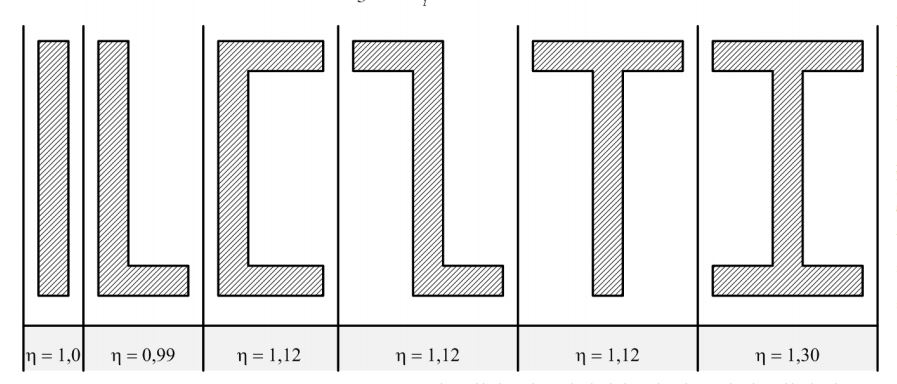
\includegraphics[scale=0.6]{Torsion_5.jpg}
\end{figure}

\begin{align*}
I_t &= \frac{1}{3} \cdot \eta \cdot \sum_{i}^{} l_i \cdot h_t^3
\end{align*}

\newpage


\section{Mechanismen}

In der Ebene gibt des 3 Freiheitsgrade, im Raum 6. Wegen dem Gestell hat man dann $b \cdot (n-1)$ Freiheitsgrade. Jedes Gelenk eliminiert $u = b - f$ Freiheitsgrade.

\begin{align*}
\intertext{Laufgrad:}
F &= b \cdot \left( n - 1 \right) - g \cdot b + \sum_{i=1}^{g} f_i \\
F &\leq -1 \qquad \text{überbestimmt, nicht montierbar} \\
F &= 0 \qquad \text{statisch bestimmt} \\
F &= 1 \qquad \text{ein Getriebeglied bewegt auch alle anderen, ein Antrieb} \\
F &\geq 1 \qquad \text{es werden F Antriebe gebraucht}
\end{align*}


\subsection*{Überbestimmtheit}

\begin{align*}
\text{Ü} &= \sum_{i=1}^{k} u_i' - u \\
\text{Ü} &= \text{Grad der Überbestimmtheit} \\
u_i' &= \text{Unfreiheitsgrad des Untergelenks i} \\
u &= \text{Vorgesehender Unfreiheitsgrad des Gesamtgelenks} \\
k &= \text{Anzahl der Untergelenke (Wirkflächenpaare)}
\end{align*}


\newpage

\section{Toleranzen}

\subsection*{Maße}

\begin{figure}[h]
	\centering
	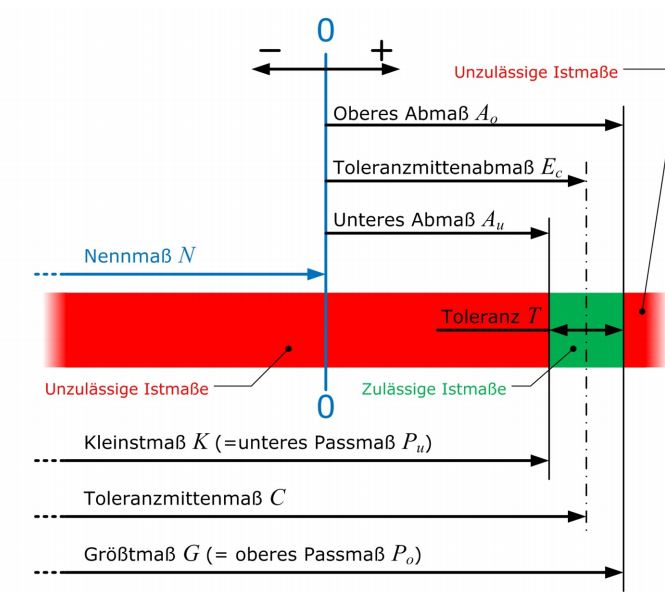
\includegraphics[scale=0.6]{Toleranzen_1.jpg}
\end{figure}

\begin{align*}
M &= N^{A_0}_{A_u} = N + E_c \pm \frac{T}{2} = N^{E_c + \frac{T}{2}}_{E_c - \frac{T}{2}} \\
G &= N + A_o = N + E_c + \frac{T}{2} \\
K &= N + A_o = N + E_c - \frac{T}{2}
\end{align*}

\newpage

\subsection*{Maßtabelle}

\begin{figure}[h]
	\centering
	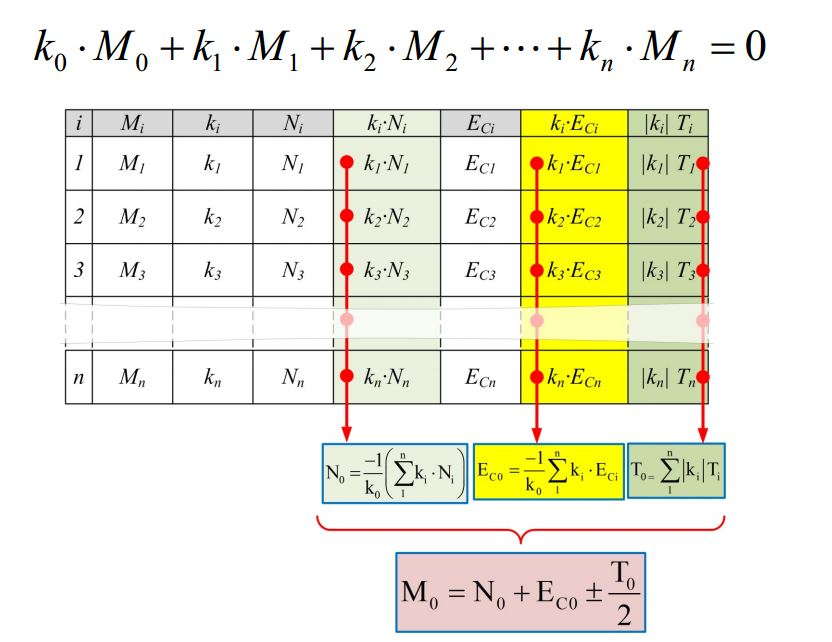
\includegraphics[scale=0.7]{Masstabelle.jpg}
\end{figure}








\end{document}